% IMPORTANT: PLEASE USE XeLaTeX FOR TYPESETTING
\documentclass{sintefbeamer}
\usepackage{xeCJK}
\usepackage{ragged2e}
\usepackage{amsthm}
\usepackage{listings}
\setbeamertemplate{theorems}[numbered]
\makeatletter
\setbeamertemplate{footline}
{
  \leavevmode%
  \hbox{%
  \begin{beamercolorbox}[wd=.7\paperwidth,ht=2.25ex,dp=1ex,center]{title in head/foot}%
    \usebeamerfont{title in head/foot} {Reproduced Analysis}
  \end{beamercolorbox}%
  \begin{beamercolorbox}[wd=.3\paperwidth,ht=2.25ex,dp=1ex,right]{date in head/foot}%
    \usebeamerfont{date in head/foot}\insertshortdate{}\hspace*{2em}
    \insertframenumber{} / \inserttotalframenumber\hspace*{2ex} 
  \end{beamercolorbox}}%
  \vskip0pt%
}

%\newtheorem{theorem}{Theorem} % to number according to section
\theoremstyle{definition}

\makeatother

% meta-data
\title{\large Reproduced Analysis for ``Integrated multimodal artificial intelligence framework for healthcare applications"}
\subtitle{Author: 黄其涵, Adviser: 毛晓伟}
\date{\today}
\titlebackground{images/bg_uestc}

% document body
\begin{document}

\maketitle


\section{Intro}

\begin{frame}{Background}

\justifying
Artificial intelligence (AI) systems hold great promise to improve healthcare over the next decades. Specifically, AI systems leveraging multiple data sources and input modalities are poised to become a viable method to deliver more accurate results and deployable pipelines across a wide range of applications [1].

\vspace{0.7cm}

\tiny [1] Soenksen, Luis R., et al. ``Integrated multimodal artificial intelligence framework for healthcare applications." \textit{NPJ digital medicine} 5.1 (2022): 149.


\end{frame}

\begin{frame}{Challenges of Single-source AI Systems}

The specific challenges faced by AI systems relying on single data sources:
\begin{enumerate}
\item Accuracy limitations in complex cases.
\item Lack of generalizability across diverse patient populations and conditions.
\item Reduced applicability in multifaceted healthcare scenarios.
\end{enumerate}

\end{frame}

\begin{frame}{Contributions of HAIM System}

\small

The contributions of Holistic AI in Medicine (HAIM) can be summarized as follows:

\begin{enumerate}
    \item This work introduced the HAIM framework, \textbf{integrating multiple data sources and modalities into a cohesive system for constructing AI applications in healthcare}.     
    \item This research shows that \textbf{multiple-source or models developed within the HAIM framework consistently outperform single-source models} across various healthcare applications, including diagnostics and prognostics. It also emphasizes \textbf{the utility of multimodal data in enhancing the accuracy and reliability of AI systems in medicine}.    
    \item \textbf{Utilizing Shapley values to quantify the contributions of each data modality and source}, this provide insights into the heterogeneity of data modality importance. 
\end{enumerate}


\end{frame}

\section{Methods}

\begin{frame}{Datasets}

\footnotesize \textbf{MIMIC-IV}: The Medical Information Mart for Intensive Care IV (MIMIC-IV) is a large database containing de-identified health-related data associated with over forty thousand patients who stayed in critical care units of the Beth Israel Deaconess Medical Center between 2008 and 2019 [2].\\[0.2cm]

\footnotesize \textbf{MIMIC-CXR-JPG}: The MIMIC Chest X-ray JPG (MIMIC-CXR-JPG) Database v2.0.0 is a large publicly available dataset of chest radiographs in JPG format with structured labels derived from free-text radiology reports. The MIMIC-CXR-JPG dataset is wholly derived from MIMIC-CXR, providing JPG format files derived from the DICOM images and structured labels derived from the free-text reports [3].\\[0.5cm]

\tiny [2] Johnson, A., Bulgarelli, L., Pollard, T., Horng, S., Celi, L. A., \& Mark, R. (2021). MIMIC-IV (version 1.0). PhysioNet. \url{https://doi.org/10.13026/s6n6-xd98}.\\[0.1cm]

\tiny [3] Johnson, A., Lungren, M., Peng, Y., Lu, Z., Mark, R., Berkowitz, S., \& Horng, S. (2019). MIMIC-CXR-JPG - chest radiographs with structured labels (version 2.0.0). PhysioNet. \url{https://doi.org/10.13026/8360-t248}.

\end{frame}

\begin{frame}{Datasets}

\footnotesize \textbf{HAIM-MIMIC-MM}: A unified multimodal dataset created by combining the MIMIC-IV v1.0 and the MIMIC-CXR-JPG database v2.0.0. This dataset mainly uses subject\_id, hadm\_id,stay\_id as the primary key to create links in the tables of each database:
\begin{itemize}
    \item \textbf{subject\_id}: Unique identifier for a patient. This ID ensures patient anonymity while allowing researchers to link different hospital visits or admissions for the same individual.
    \item \textbf{hadm\_id}: Unique identifier for a patient's hospital admission. This ID is used to differentiate between multiple admissions for the same patient, facilitating the study of each separate hospital stay.
    \item \textbf{stay\_id}: Unique identifier for a patient's stay in a specific ward or ICU during a hospital admission. It allows for the analysis of patient care at a more granular level, focusing on individual segments of the hospital stay.
\end{itemize}
\end{frame}

\begin{frame}[fragile]{Datasets}

\footnotesize
The final HAIM data unit object ->
\begin{lstlisting}[language=Python]
class Patient_ICU(object):
    def __init__(self, admissions, demographics, transfers, core,
        diagnoses_icd, drgcodes, emar, emar_detail, hcpcsevents,
        labevents, microbiologyevents, poe, poe_detail,
        prescriptions, procedures_icd, services, procedureevents,
        outputevents, inputevents, icustays, datetimeevents,
        chartevents, cxr, imcxr, noteevents, dsnotes, ecgnotes,
        echonotes, radnotes):

## CORE
self.admissions = admissions  # Patient admissions information
self.demographics = demographics  # Patient demographics data
self.transfers = transfers # Patient transfer data within hospital
self.core = core  # Core patient information

\end{lstlisting}
\end{frame}

\begin{frame}[fragile]{Datasets}

\begin{lstlisting}[language=Python]
## HOSP
self.diagnoses_icd = diagnoses_icd  # Diagnoses in ICD format
self.drgcodes = drgcodes  # DRG codes for billing and reimbursements
self.emar = emar # Electronic Medication Administration Record
self.emar_detail = emar_detail 
# Detailed medication administration data
self.hcpcsevents = hcpcsevents 
# Healthcare Common Procedure Coding events
self.labevents = labevents  # Laboratory test results
self.microbiologyevents = microbiologyevents 
# Microbiology test results
self.poe = poe  # Physician Order Entry records
self.poe_detail = poe_detail # Detailed Physician Order Entry records
self.prescriptions = prescriptions # Prescribed medications
self.procedures_icd = procedures_icd # Procedures coded in ICD format
self.services = services  # Services provided to the patient 
\end{lstlisting}
\end{frame}

\begin{frame}[fragile]{Datasets}

\begin{lstlisting}[language=Python]
## ICU
self.procedureevents = procedureevents  # Procedures performed in ICU
self.outputevents = outputevents  # Outputs like fluids measured
self.inputevents = inputevents # Inputs like medications administered
self.icustays = icustays  # Information on each ICU stay
self.datetimeevents = datetimeevents  # Timestamped events
self.chartevents = chartevents  # Charted events like vital signs

## CXR
self.cxr = cxr  # Chest X-ray data
self.imcxr = imcxr  # Image data from chest X-rays

## NOTES
self.noteevents = noteevents  # Clinical notes
self.dsnotes = dsnotes  # Discharge summaries or other clinical notes
self.ecgnotes = ecgnotes  # Electrocardiogram notes
self.echonotes = echonotes  # Echocardiogram notes
self.radnotes = radnotes  # Radiology reports and notes
        
\end{lstlisting}
\end{frame}

\begin{frame}{Data Preprocessing}
\small
The generation of embeddings from input modalities encompasses a diverse range of data types. These modalities and their respective embeddings include:
\begin{itemize}
    \item \textbf{Tabular Data:} Demographics (\(E_{de}\)) are represented as tabular data.
    \item \textbf{Structured Time-Series Events:} 
    \begin{itemize}
        \item Chart events (\(E_{ce}\)),
        \item Laboratory events (\(E_{le}\)),
        \item Procedure events (\(E_{pe}\)).
    \end{itemize}
    \item \textbf{Unstructured Free Text:} 
    \begin{itemize}
        \item Radiological notes (\(E_{radn}\)),
        \item Electrocardiogram notes (\(E_{ecgn}\)),
        \item Echocardiogram notes (\(E_{econ}\)).
    \end{itemize}
    \item \textbf{Single-Image Vision:} 
    \begin{itemize}
        \item Visual probabilities (\(E_{vp}\)),
        \item Visual dense-layer features (\(E_{vd}\)).
    \end{itemize}
    
\end{itemize}
\end{frame}

\begin{frame}{Data Preprocessing}
\small
\begin{itemize}
    
    \item \textbf{Multi-Image Vision:} 
    \begin{itemize}
        \item Aggregated visual probabilities (\(E_{vmp}\)),
        \item Aggregated visual dense-layer features (\(E_{vmd}\)).
    \end{itemize}
\end{itemize}
\begin{figure}[htbp]
  \centering
  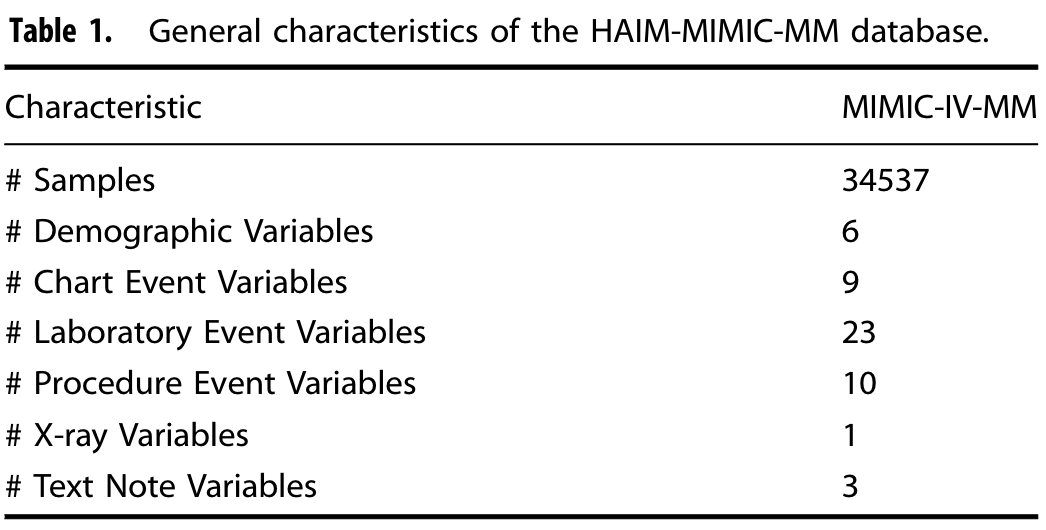
\includegraphics[width=0.7\textwidth]{images/table1}
%  \caption{\scriptsize An example of trajectory generation.}
  \label{fig:ex1}	
\end{figure}
\end{frame}

\begin{frame}{DataFrame Embeddings}
\footnotesize

The following data frames contain embeddings extracted from various patient data, where each prefix in the column names represents the type of embedding:

\begin{itemize}
  \item \texttt{df\_demographics\_embeddings\_fusion}: Contains embeddings from demographic information of patients. Prefix \texttt{de\_} stands for \emph{demographics embeddings}.
  
  \item \texttt{df\_ts\_ce\_embeddings\_fusion}: Contains time-series feature embeddings extracted from chart events of patients. Prefix \texttt{ts\_ce\_}  stands for \emph{time series chart events}.
  
  \item \texttt{df\_ts\_le\_embeddings\_fusion}: Contains time-series feature embeddings extracted from laboratory events of patients. Prefix \texttt{ts\_le\_} stands for \emph{time series lab events}.
  
  \item \texttt{df\_ts\_pe\_embeddings\_fusion}: Contains time-series feature embeddings extracted from procedure events of patients. Prefix \texttt{ts\_pe\_}  stands for \emph{time series procedure events}.
  
  \item \texttt{df\_vision\_dense\_embeddings\_fusion}: Contains dense feature embeddings extracted from single chest X-ray images. Prefix \texttt{vd\_}  stands for \emph{vision dense}.

\end{itemize}

\end{frame}


\begin{frame}{DataFrame Embeddings}
\footnotesize

\begin{itemize}

  
  \item \texttt{df\_vision\_predictions\_embeddings\_fusion}: Contains predictive feature embeddings extracted from single chest X-ray images. Prefix \texttt{vp\_}  stands for \emph{vision predictions}.
  
  \item \texttt{df\_vision\_multi\_dense\_embeddings\_fusion}: Contains dense feature embeddings accumulated from multiple chest X-ray images. Prefix \texttt{vmd\_}  stands for \emph{vision multi dense}.
  
  \item \texttt{df\_vision\_multi\_predictions\_embeddings\_fusion}: Contains predictive feature embeddings accumulated from multiple chest X-ray images. Prefix \texttt{vmp\_} likely stands for \emph{vision multi predictions}.
  
  \item \texttt{df\_ecgnotes\_embeddings\_fusion}: Contains embeddings extracted from ECG notes. Prefix \texttt{n\_ecg\_} stands for \emph{notes ECG}.
  
  \item \texttt{df\_echonotes\_embeddings\_fusion}: Contains embeddings extracted from echocardiogram notes. Prefix \texttt{n\_ech\_}  stands for \emph{notes echocardiogram}.
  
  \item \texttt{df\_radnotes\_embeddings\_fusion}: Contains embeddings extracted from radiology reports. Prefix \texttt{n\_rad\_} stands for \emph{notes radiology}.
\end{itemize}

\end{frame}

\begin{frame}[fragile]{Modeling}{Length of Stay Modeling}
\small
This work framed the prediction of patient discharge within the next 48 hours as a binary classification problem: discharged alive within 48 hours (1) or otherwise (0). Each sample in this predictive task corresponds to a single patient-admission EHR time point where an X-ray image was obtained (N = 45,050).
\begin{lstlisting}[language=Python]
Main function:
    # load the HAIM embedding file
    fname = 'data/cxr_ic_fusion.csv'
    df = pd.read_csv(fname, skiprows=[45051, 45052])    
    # Tagging and labelling
    df_alive_small48 = df[((df['img_length_of_stay'] < 48) & (df['death_status'] == 0))]
    df_alive_big48 = df[((df['img_length_of_stay'] >= 48) & (df['death_status'] == 0))]
    df_death = df[(df['death_status'] == 1)]
    df_alive_small48['y'] = 1
    df_alive_big48['y'] = 0
    df_death['y'] = 0 
    df = pd.concat([df_alive_small48, df_alive_big48, df_death], axis=0)
\end{lstlisting}
\end{frame}

\begin{frame}[fragile]{Modeling}{Length of Stay Modeling}
\small
\begin{lstlisting}[language=Python]
Main function:
    ......
    # Remove unnecessary columns
    df = df.drop(['img_id', 'img_charttime', 'img_deltacharttime', 'discharge_location', 'img_length_of_stay',
                  'death_status'], axis=1)
    
    # Get all types of data sources, 'de_', 'vd_', 'vp_', 'vmd_',...
    data_type_dict = get_data_dict(df)
    
    # Combine and arrange all types of input samples
    all_types_experiment = get_all_dtypes()

    # Number of Cases:  2047
    # Run multithreaded execution task
    results = parallel_run(all_types_experiment, data_type_dict, df, 'lengthOfStay', start_index=22)
\end{lstlisting}
\end{frame}

\begin{frame}[fragile]{Modeling}{Length of Stay Modeling}
\small
This function is designed to run a grid search with cross-validation on a set of hyperparameters for the XGBoost classifier, optimizing for the ROC AUC metric.
\begin{lstlisting}[language=Python]
def run_xgb(x_train, y_train, x_test):
    cv_folds = 5
    gs_metric = 'roc_auc'
    param_grid = {'max_depth': [5, 6, 7, 8],
                  'n_estimators': [200, 300],
                  'learning_rate': [0.3, 0.1, 0.05],}

    est = xgb.XGBClassifier(verbosity=0, scale_pos_weight=(len(y_train) - sum(y_train)) / sum(y_train), seed=42,
                            tree_method='hist', gpu_id=0, eval_metric='logloss')

    gs = GridSearchCV(estimator=est, param_grid=param_grid, scoring=gs_metric, cv=cv_folds)
    gs.fit(x_train, y_train)
    ......
    
\end{lstlisting}
\end{frame}

\begin{frame}[fragile]{Modeling}{Mortality Prediction Modeling}
\small
This work predicted if a patient would pass away within the next 48 hours, treating it as a binary classification: expiring within 48 hours (1) or not (0). For patients not marked for expiration, the class label is 0.

\begin{lstlisting}[language=Python]
Main function:
    ......
    fname = 'data/cxr_ic_fusion.csv'
    df = pd.read_csv(fname, skiprows=[45051, 45052])

    df_death_small48 = df[((df['img_length_of_stay'] < 48) & (df['death_status'] == 1))]
    df_alive_big48 = df[((df['img_length_of_stay'] >= 48) & (df['death_status'] == 0))]
    df_death_big48 = df[((df['img_length_of_stay'] >= 48) & (df['death_status'] == 1))]

    df_death_small48['y'] = 1
    df_alive_big48['y'] = 0
    df_death_big48['y'] = 0
    ......
\end{lstlisting}


\end{frame}

\begin{frame}{Modeling}{Pathology Diagnosis Modeling}
\small
This work targeted predicting 10 common chest pathologies (e.g., fractures, lung lesions) using the HAIM framework, which showed superior performance over image-only methods. The dataset for this study, derived from MIMIC-CXR-JPG v2.0.0, labeled pathologies as present (1), absent (0), or inconclusive (-1); we excluded inconclusive cases. Excluding unstructured radiology notes to prevent overfitting, we utilized multimodal inputs for binary classification of each pathology. Sample sizes varied by pathology, with totals ranging from 557 (Fracture) to 18,571 (Cardiomegaly).
\end{frame}


\section{Results}

\begin{frame}{Multi-source vs. Single-source}{Length of Stay Modeling}

\begin{figure}[htbp]
  \centering
  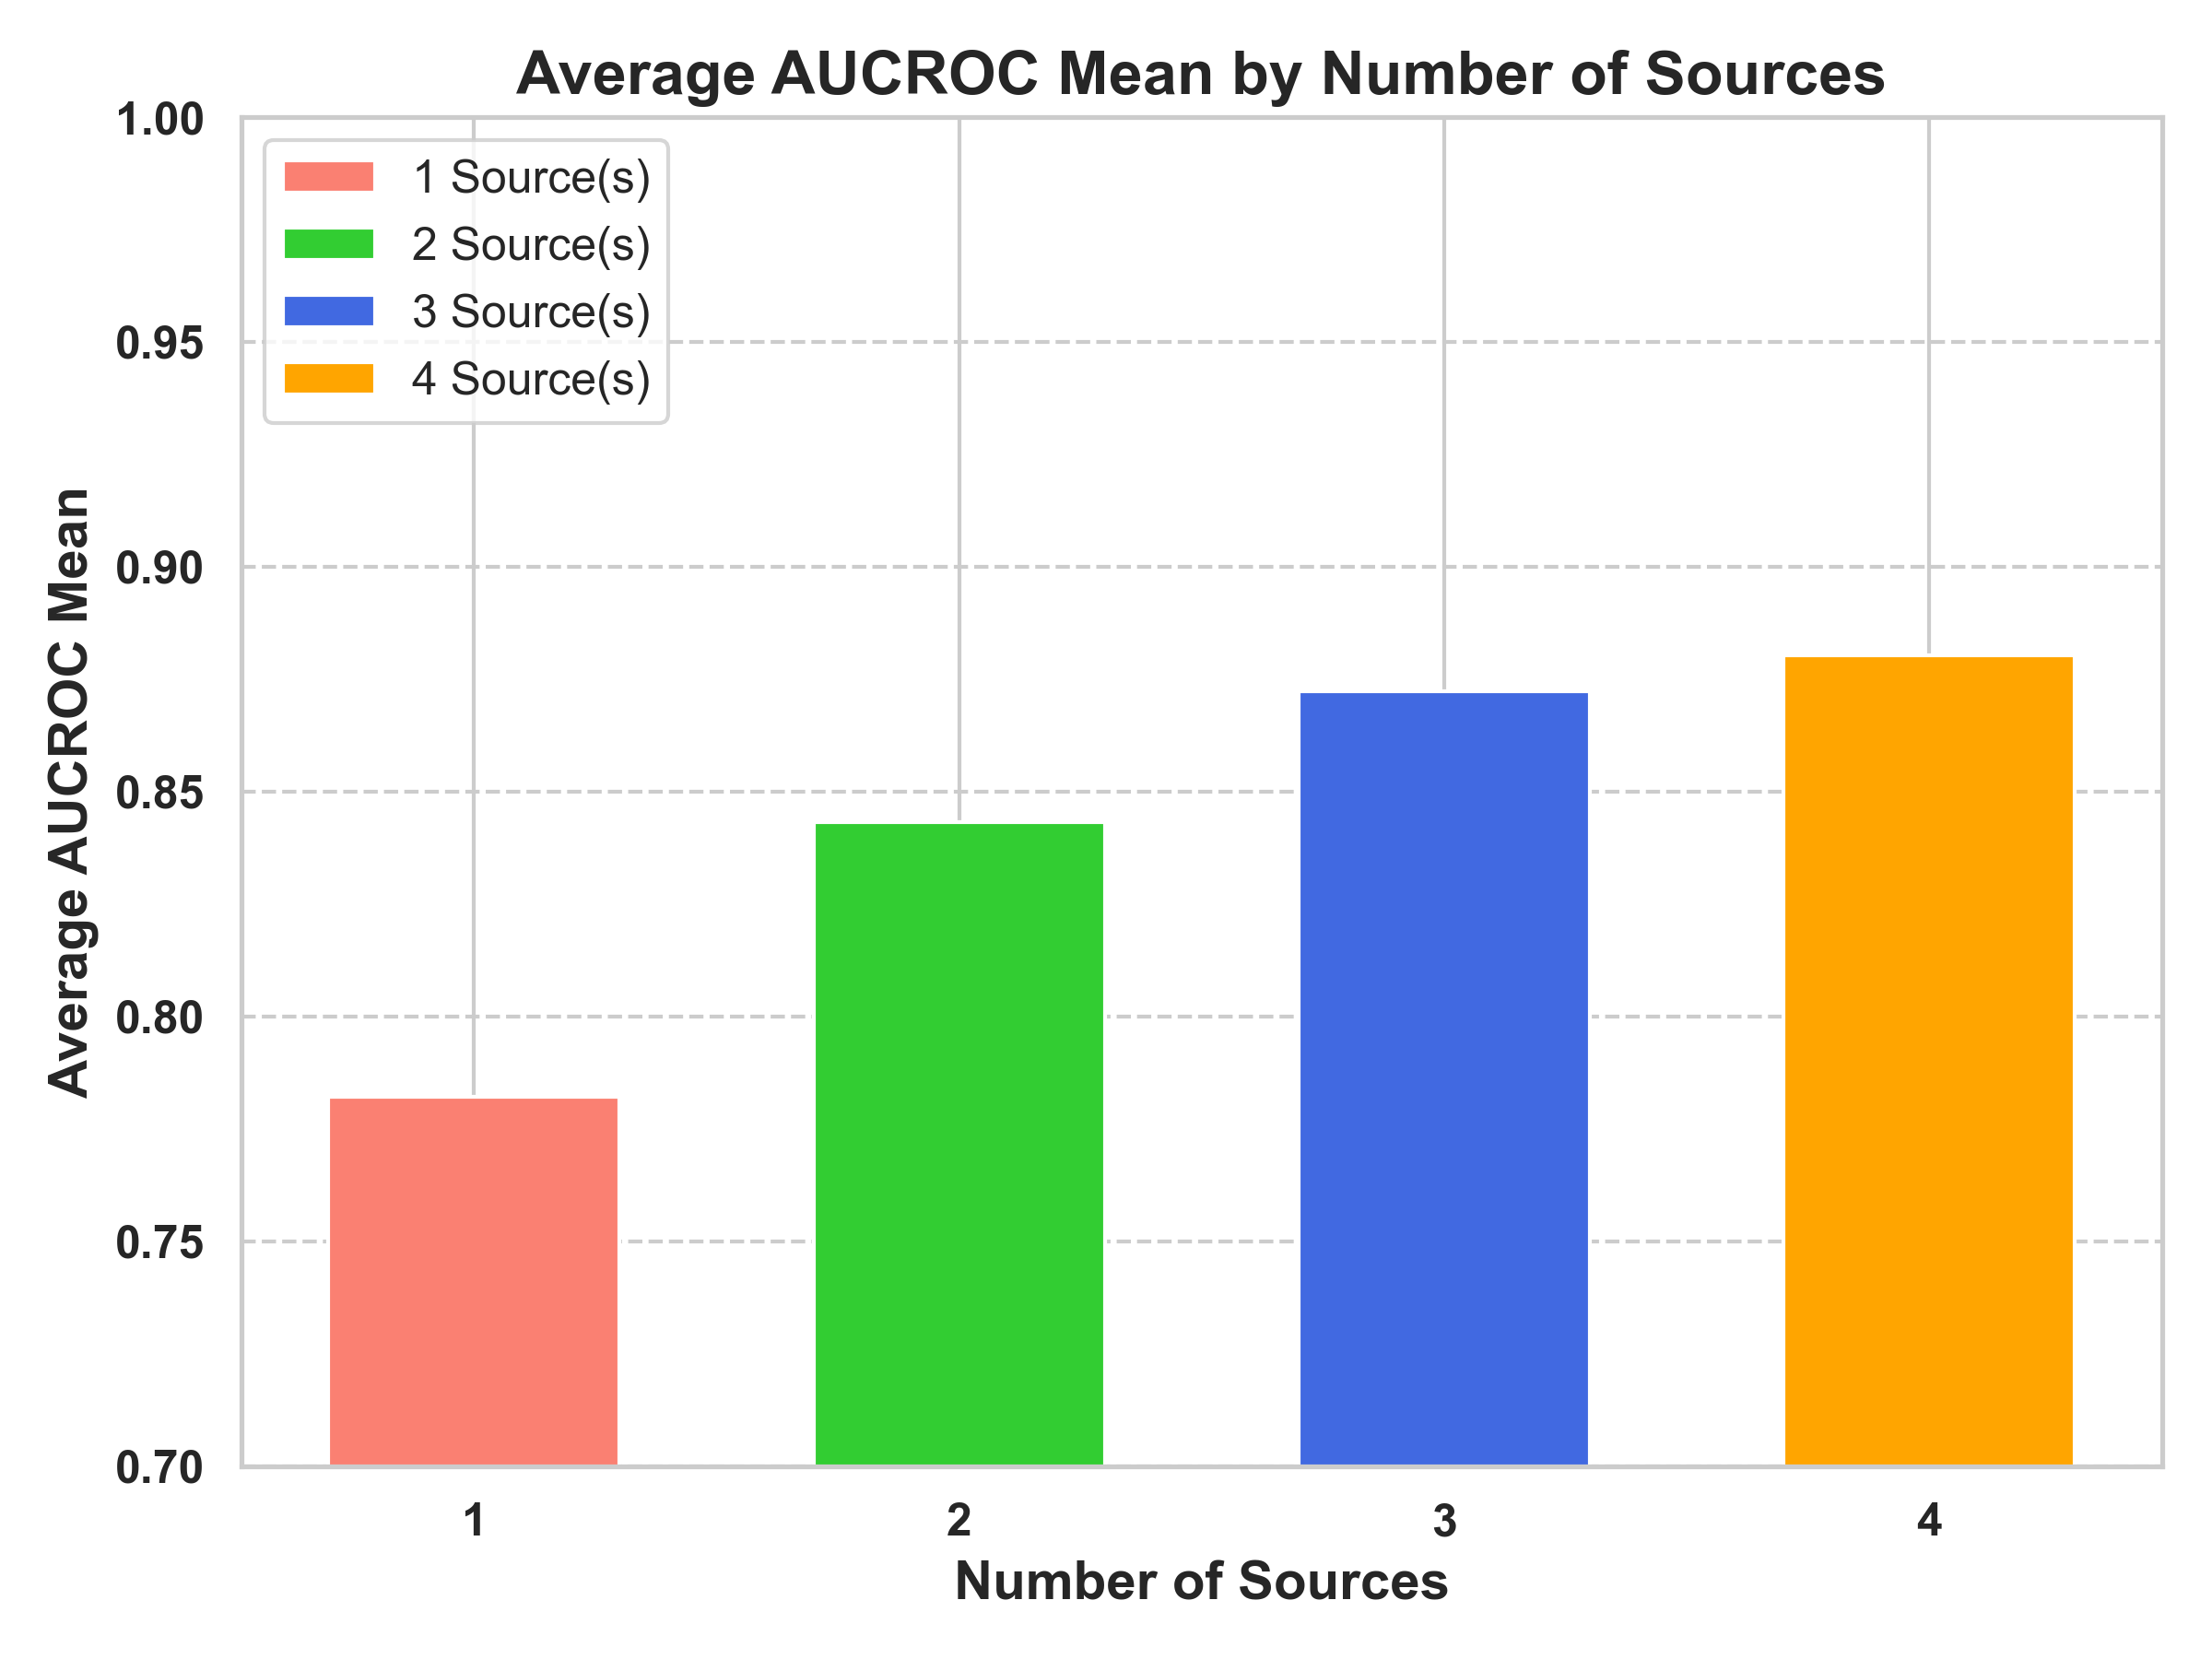
\includegraphics[width=0.7\textwidth]{images/average_auc_by_sources.png}
%  \caption{\scriptsize An example of trajectory generation.}
  \label{fig:ex1}	
\end{figure}
\end{frame}

\begin{frame}{Multimodality vs. Single Modality}{Length of Stay Modeling}


\begin{figure}[htbp]
  \centering
  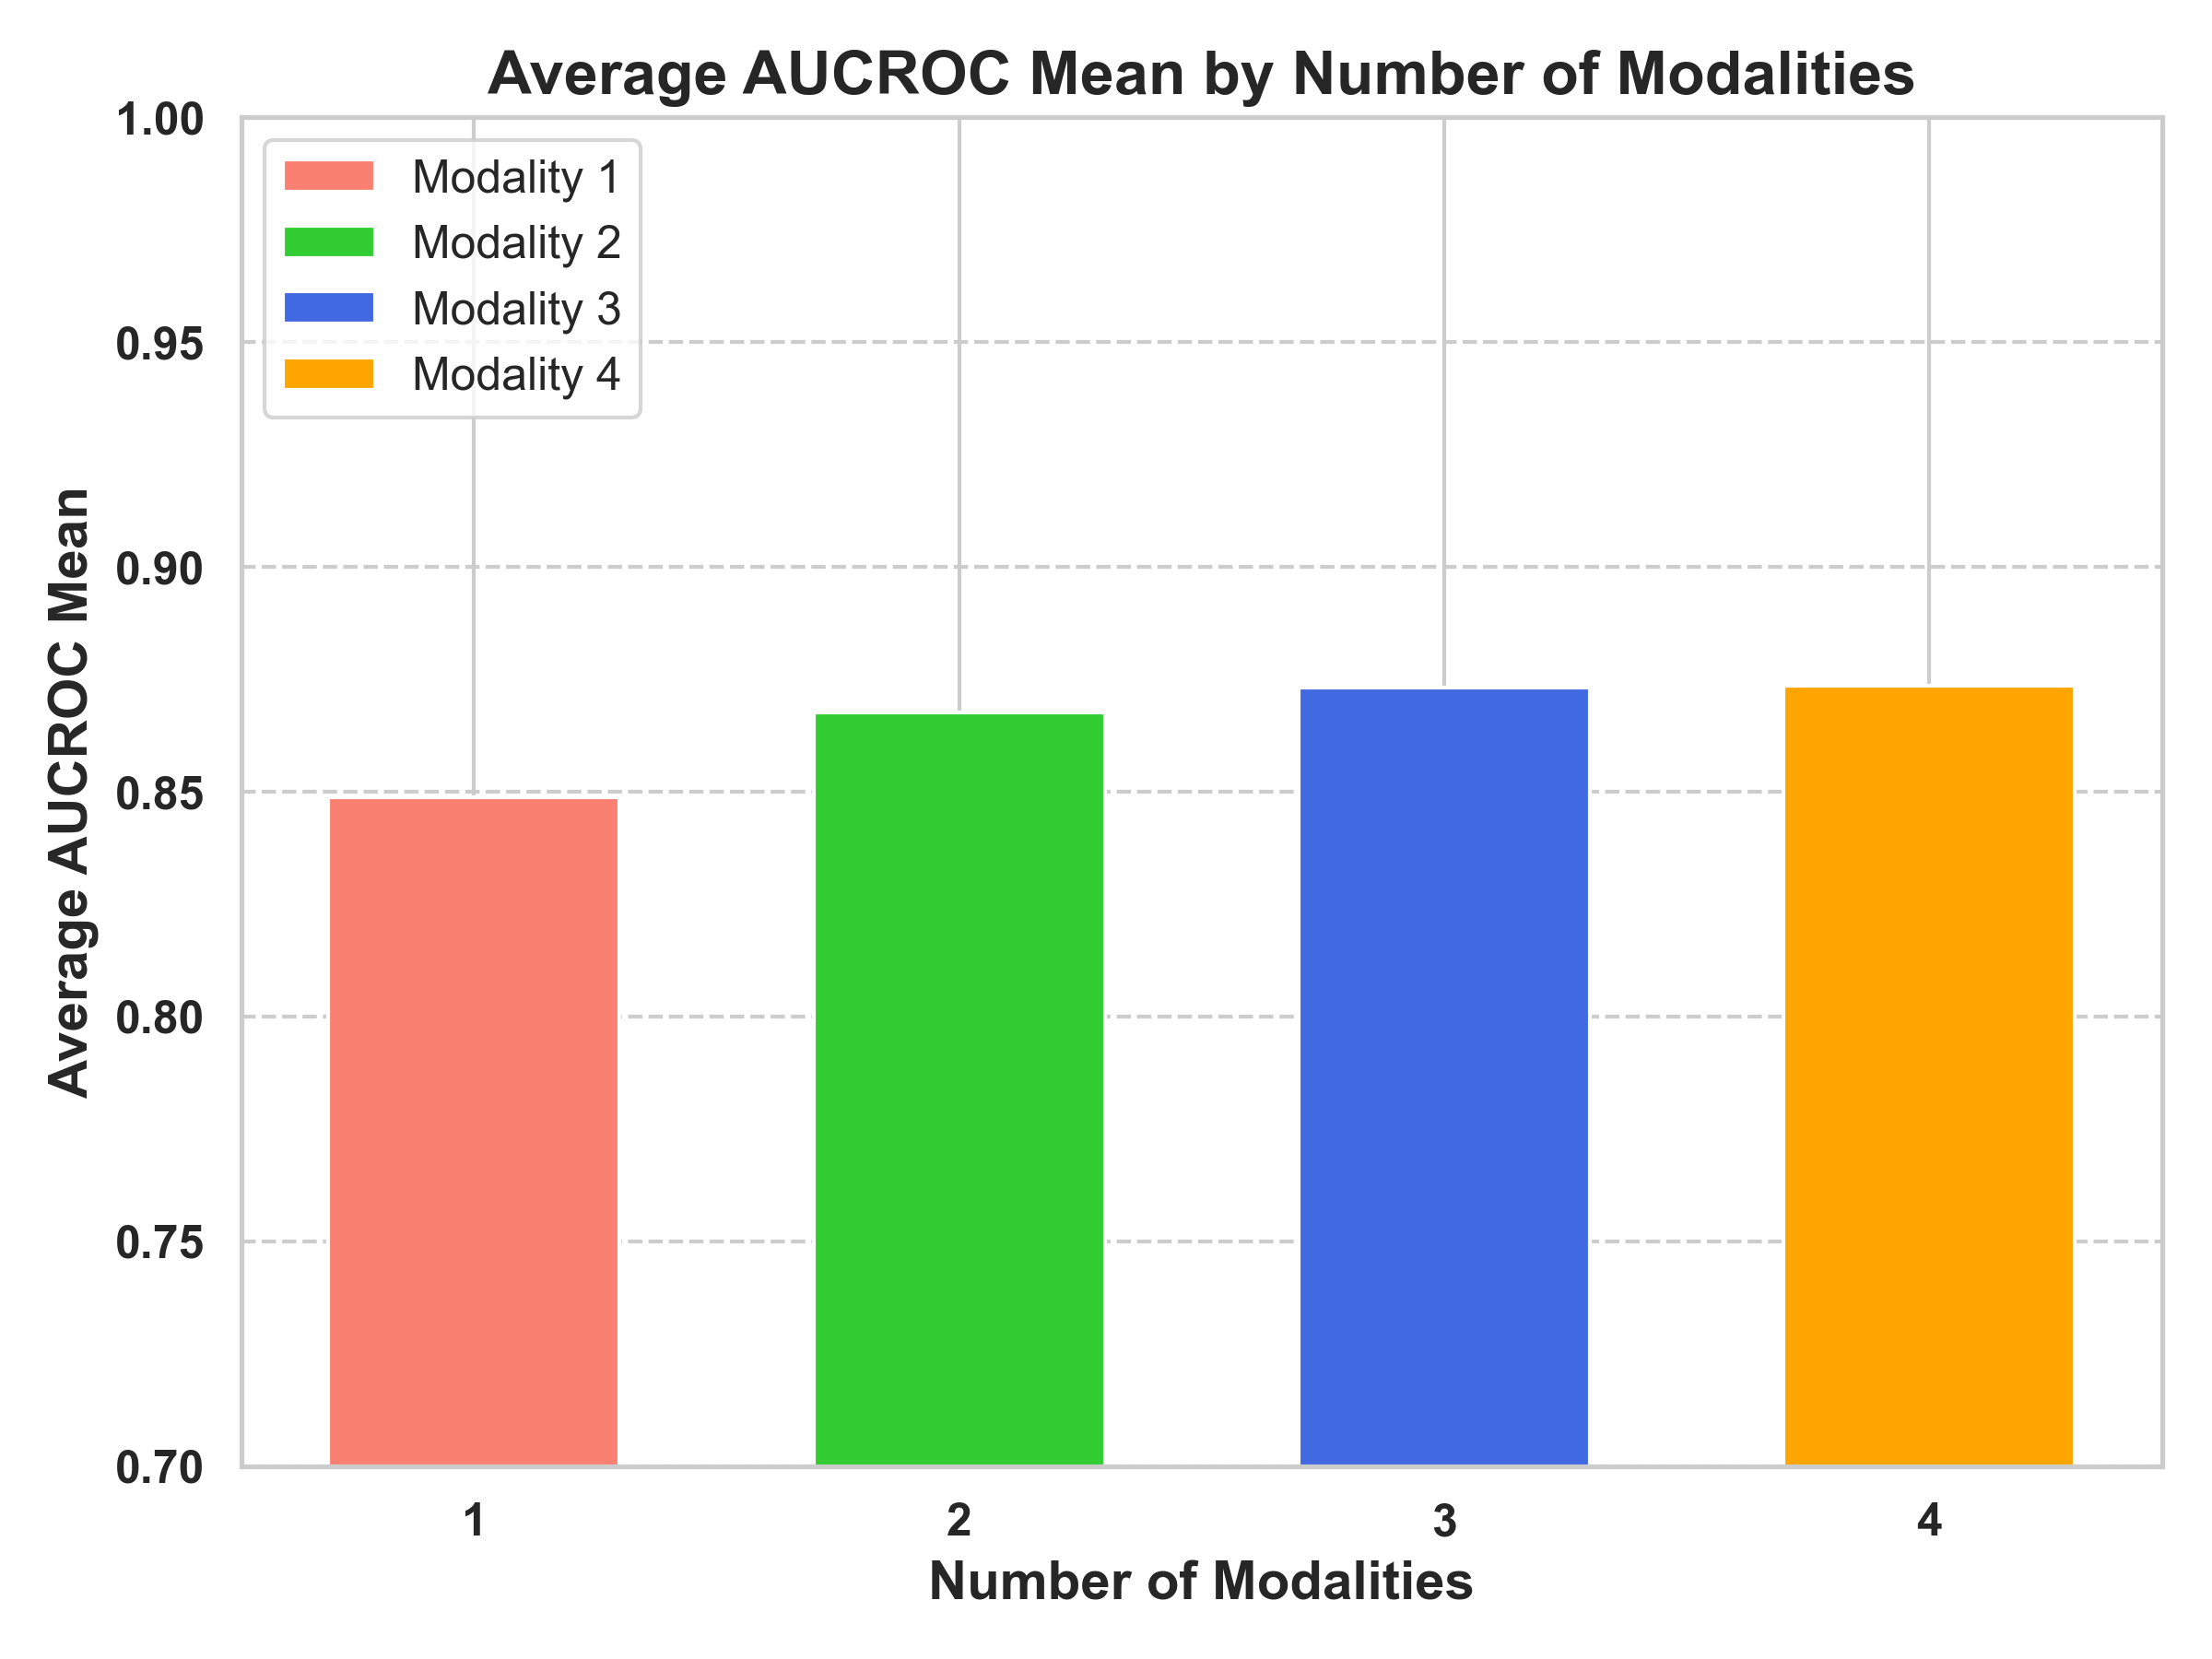
\includegraphics[width=0.7\textwidth]{images/average_auc_by_modalities.png}
%  \caption{\scriptsize An example of trajectory generation.}
  \label{fig:ex1}	
\end{figure}
\end{frame}

%\begin{frame}{ Quantification by Shapley Values}{Formula}
%
%
%
%\end{frame}


\begin{frame}{Quantification by Shapley Values}{Length of Stay Modeling}
\begin{figure}[htbp]
  \centering
  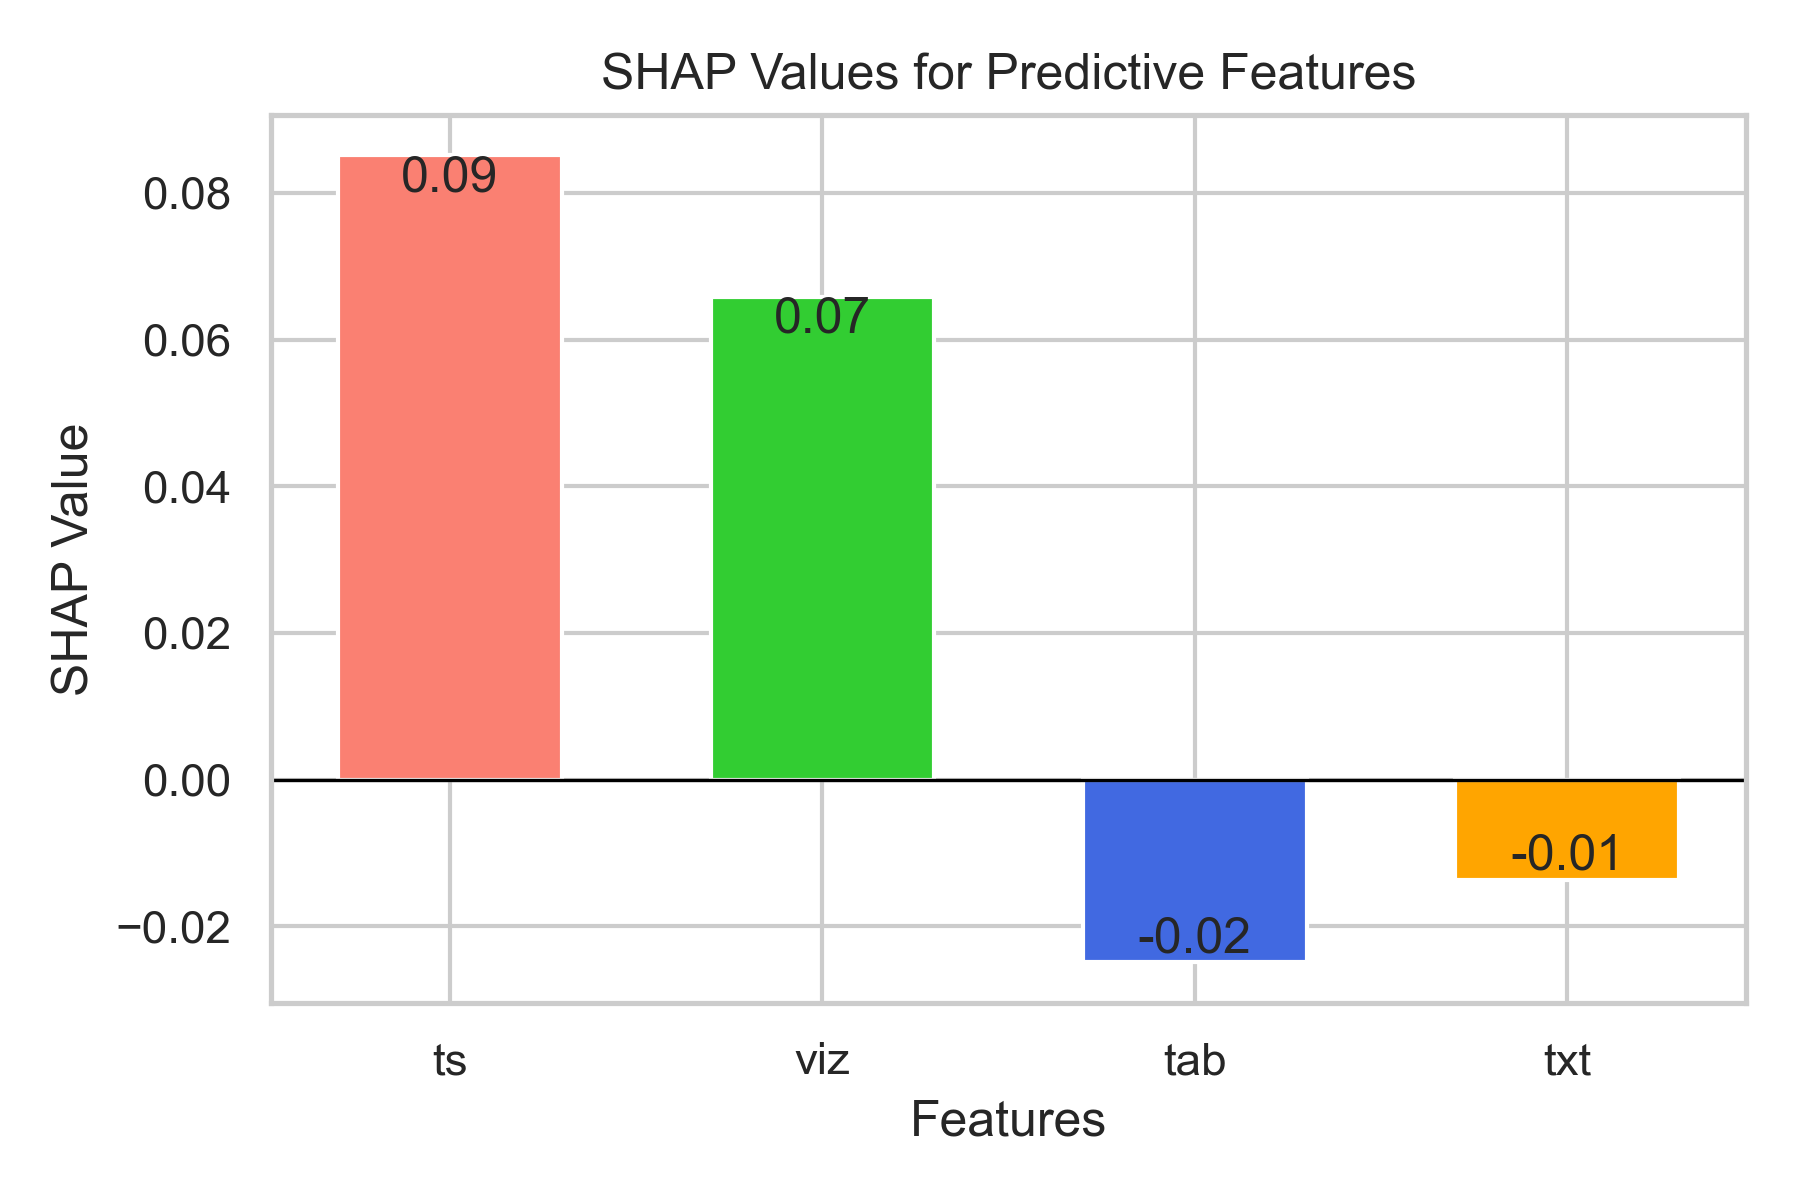
\includegraphics[width=0.7\textwidth]{images/shap_value_los.png}
%  \caption{\scriptsize An example of trajectory generation.}
  \label{fig:ex1}	
\end{figure}
\end{frame}
\backmatter
\end{document}
